%============================================================
%  Capitolo 12 -- Transformers
%  Basato sulle slide di Vito Walter Anelli (Politecnico di Bari)
%  Riferimento: Vaswani et al., "Attention is All You Need", 2017
%============================================================
\chapter{Transformers}
\label{ch:transformers}

L'architettura \textbf{Transformer}, introdotta da Vaswani et al.\ nel
2017 con il titolo \emph{Attention is All You Need}, ha rivoluzionato
il deep learning per sequenze eliminando la ricorrenza e la convoluzione
a favore di un meccanismo puramente basato sull'\emph{attention}.
Il modello risultante e' altamente parallelizzabile, cattura dipendenze
a lungo raggio in modo diretto ed e' diventato la base di quasi tutti
i modelli linguistici moderni \citep{bishop2024}.

%------------------------------------------------------------
\section{Architettura ad Alto Livello}
\label{sec:transformer-overview}

\subsection{Stack Encoder--Decoder}
\label{subsec:enc-dec}

Nella formulazione originale per la traduzione automatica, il
Transformer e' composto da due moduli:

\begin{description}
  \item[Stack di Encoder] Una sequenza di $N = 6$ encoder identici
        in struttura ma con pesi indipendenti.
        Ogni encoder riceve la sequenza intera e produce una
        rappresentazione contestualizzata di ciascun token.
  \item[Stack di Decoder] Una sequenza di $N = 6$ decoder che generano
        la sequenza di output un token alla volta, condizionandosi
        sulle rappresentazioni prodotte dall'encoder.
\end{description}

\begin{figure}[H]
  \centering
  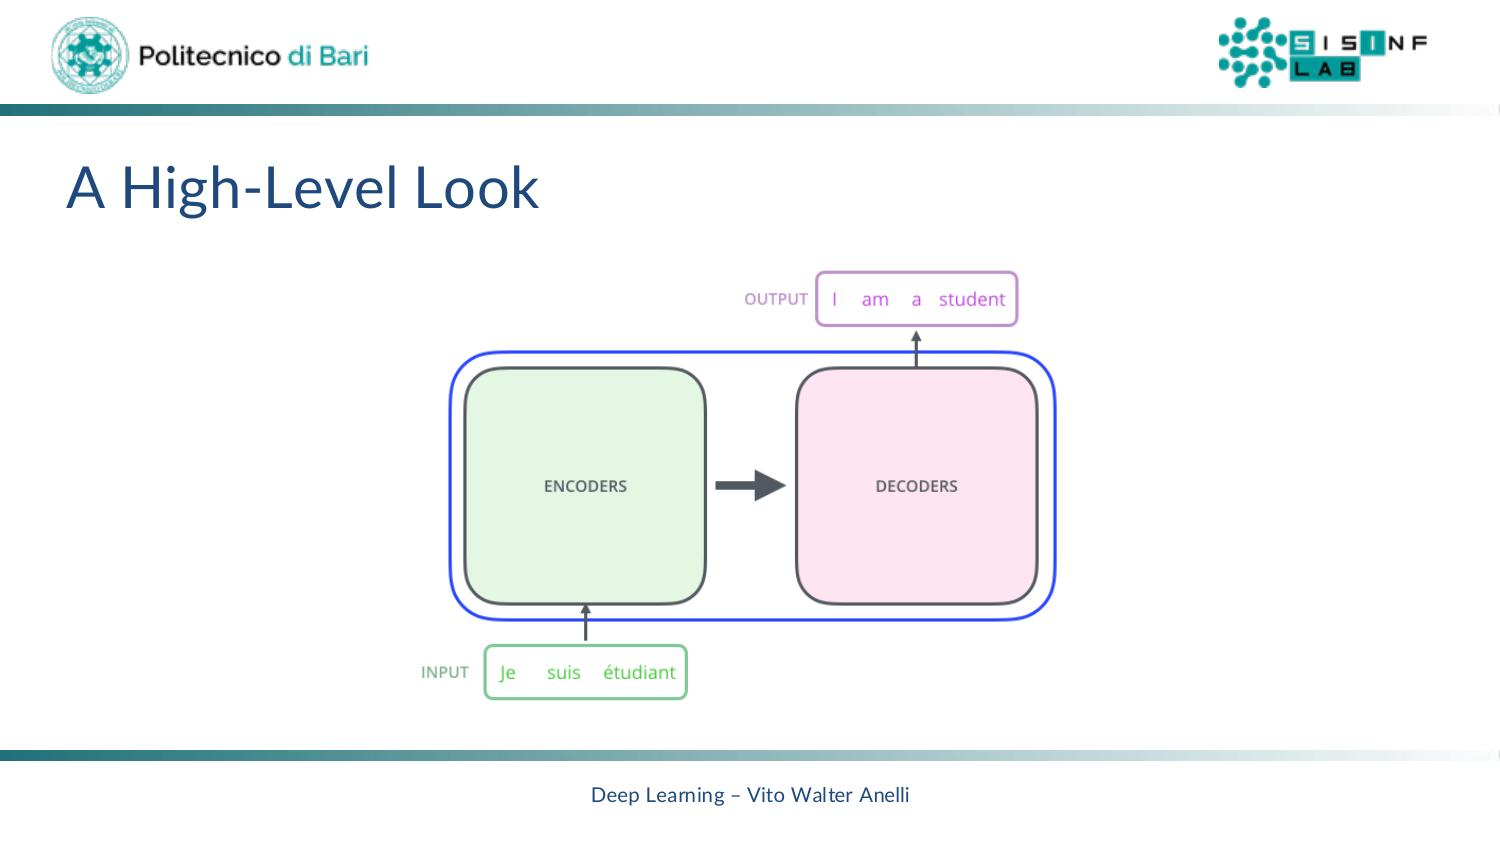
\includegraphics[width=0.62\linewidth]{figures/cf12_01_highlevel_enc_dec.jpg}
  \caption{Vista ad alto livello del Transformer. La frase di input
           (es.\ francese) attraversa lo stack di encoder; la
           rappresentazione prodotta alimenta lo stack di decoder che
           genera la traduzione (es.\ inglese) token per token.}
  \label{fig:highlevel_enc_dec}
\end{figure}

\subsection{Struttura Interna dell'Encoder}
\label{subsec:encoder-internal}

Ogni encoder e' composto da due sotto-livelli in cascata:

\begin{enumerate}
  \item \textbf{Self-Attention}: consente a ogni posizione di guardare
        tutte le altre posizioni durante la codifica, integrando il
        contesto globale nella rappresentazione di ciascun token.
        Le dipendenze tra percorsi esistono solo qui.
  \item \textbf{Feed-Forward Neural Network (FFN)}: applicata
        indipendentemente e identicamente a ciascuna posizione;
        non introduce dipendenze tra posizioni diverse, quindi i
        percorsi possono essere eseguiti in parallelo.
\end{enumerate}

\begin{figure}[H]
  \centering
  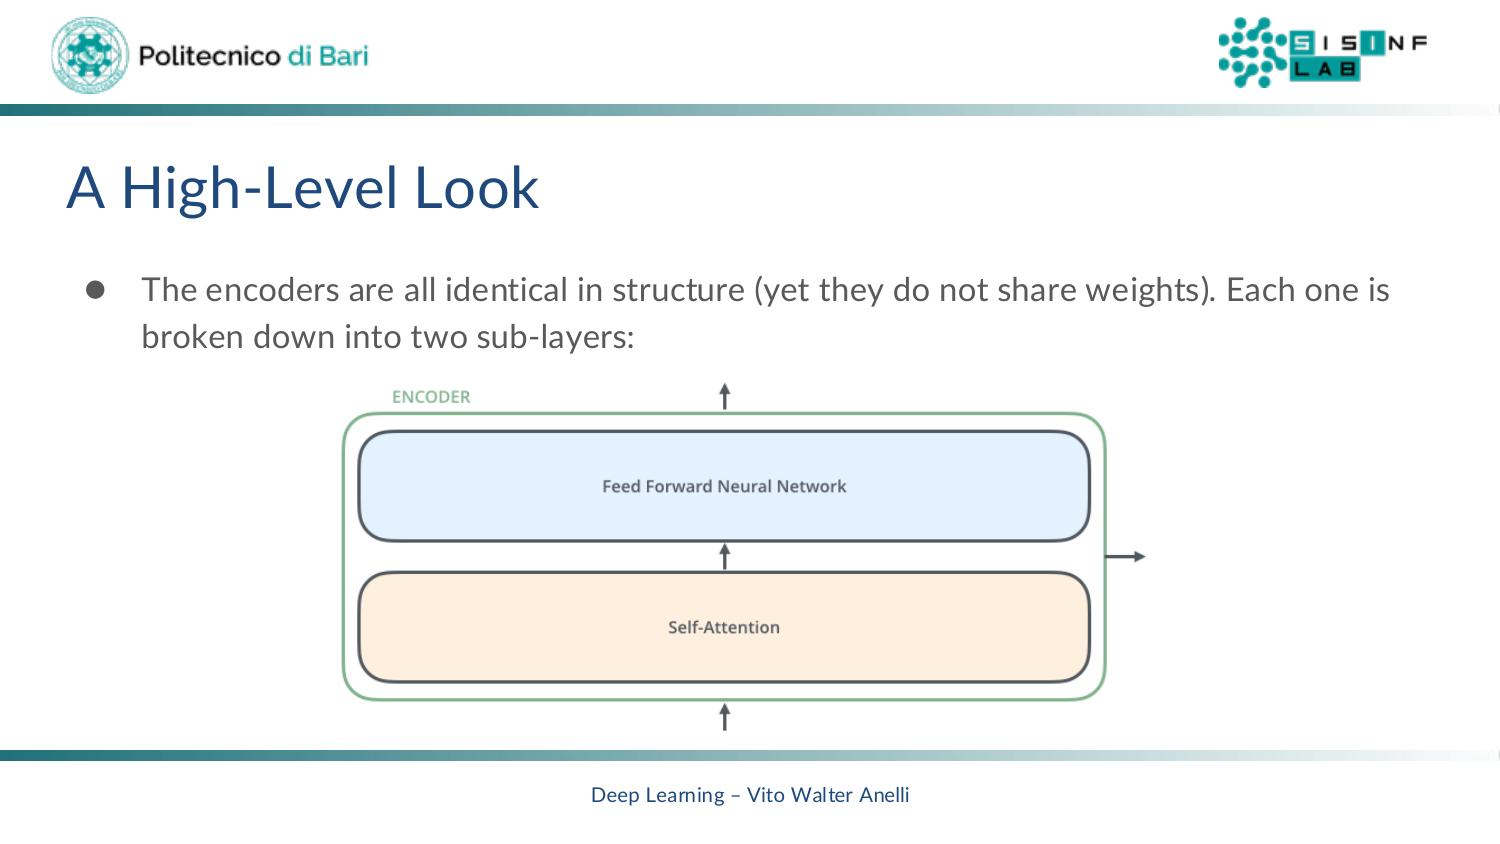
\includegraphics[width=0.60\linewidth]{figures/cf12_02_encoder_sublayers.jpg}
  \caption{Struttura interna di un singolo encoder: Self-Attention
           (rosa, sotto) produce rappresentazioni contestuali che vengono
           poi elaborate dal Feed-Forward Network (azzurro, sopra).}
  \label{fig:encoder_sublayers}
\end{figure}

\subsection{Struttura del Decoder}
\label{subsec:decoder-internal}

Il decoder aggiunge un terzo sotto-livello tra self-attention e FFN:
lo strato di \textbf{Encoder-Decoder Attention}, che consente al decoder
di focalizzarsi sulle parti rilevanti della sequenza di input. La
self-attention nel decoder e' \emph{mascherata}: ogni posizione puo'
attendere solo alle posizioni precedenti, preservando la causalita'.

\begin{figure}[H]
  \centering
  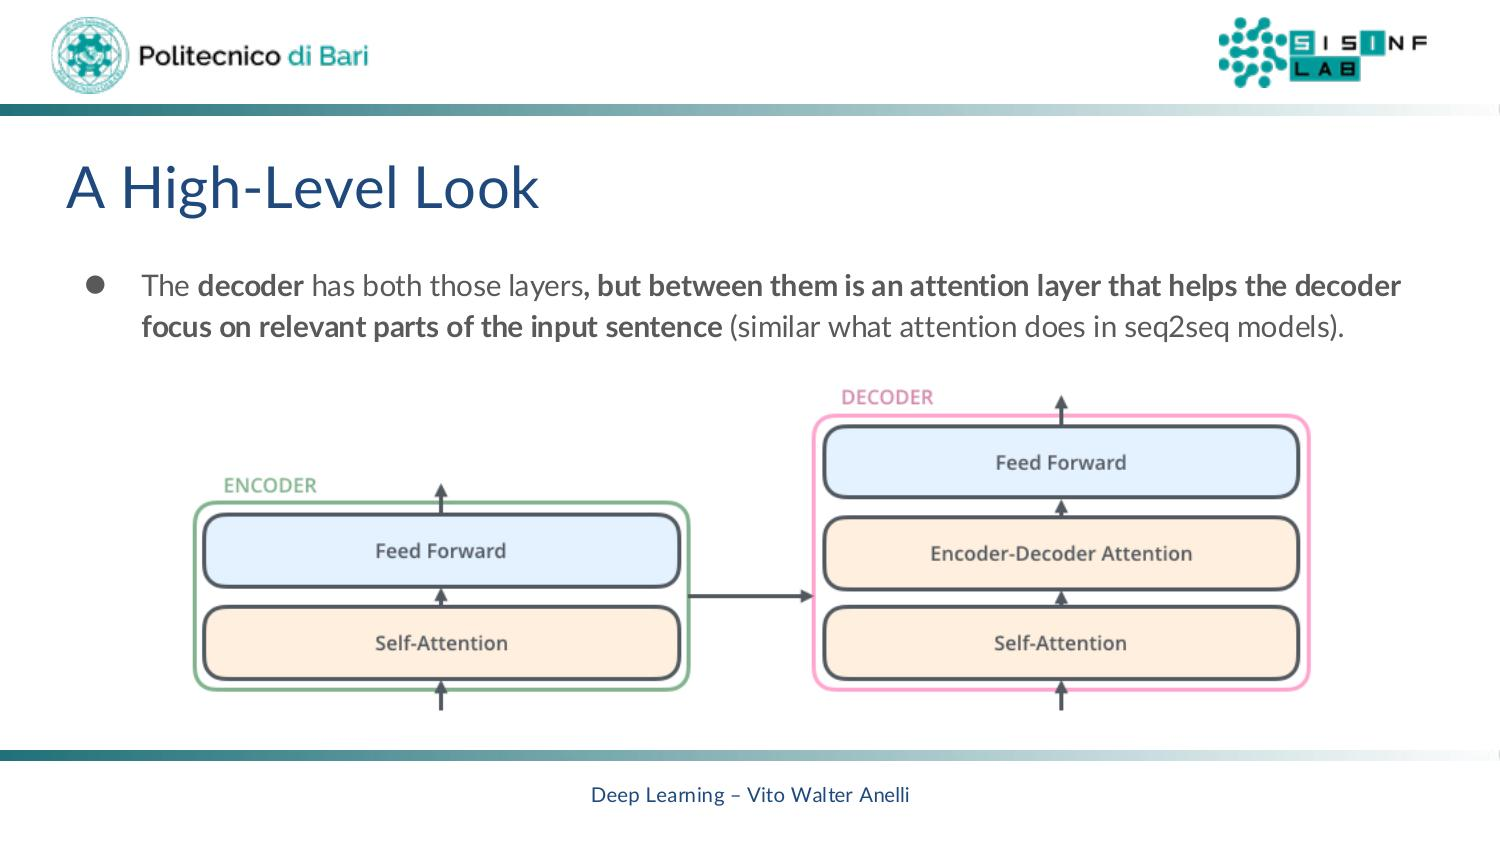
\includegraphics[width=0.82\linewidth]{figures/cf12_03_enc_dec_compare.jpg}
  \caption{Confronto tra encoder (sinistra, due sotto-livelli:
           Self-Attention + FFN) e decoder (destra, tre sotto-livelli:
           Masked Self-Attention, Encoder-Decoder Attention, FFN).
           L'Encoder-Decoder Attention riceve K e V dall'encoder.}
  \label{fig:enc_dec_compare}
\end{figure}

\subsection{Flusso dei Tensori}
\label{subsec:tensor-flow}

Prima di entrare nel primo encoder ogni token viene trasformato in un
vettore di dimensione $d_{\text{model}} = 512$ tramite una matrice
di embedding. Nei livelli successivi l'input e' l'output dell'encoder
precedente, sempre di dimensione $d_{\text{model}}$.

\begin{figure}[H]
  \centering
  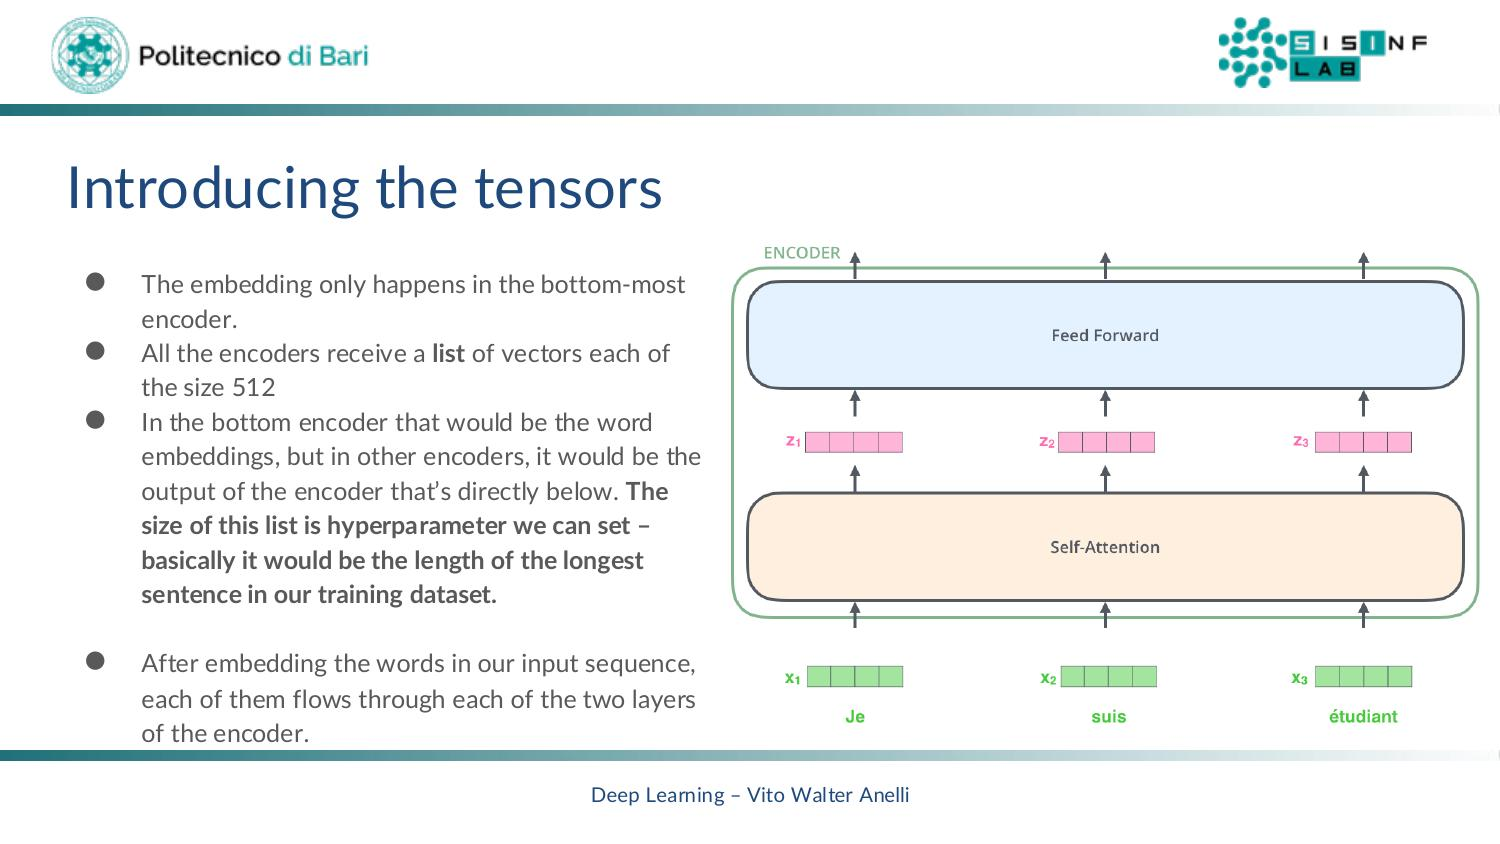
\includegraphics[width=0.78\linewidth]{figures/cf12_04_tensor_flow.jpg}
  \caption{Flusso dei tensori in un encoder. Ogni token $x_i$ (vettore
           di dimensione 512) scorre lungo il proprio percorso
           indipendente. La Self-Attention introduce dipendenze tra
           percorsi (vettori $z_i$ connessi); il FFN li processa in
           parallelo.}
  \label{fig:tensor_flow}
\end{figure}

%------------------------------------------------------------
\section{Self-Attention}
\label{sec:self-attention}

\subsection{Query, Key, Value}
\label{subsec:qkv}

Per ogni token $i$ si calcolano tre vettori tramite proiezione
lineare dell'embedding $\mathbf{x}_i$:

\begin{align}
  \mathbf{q}_i &= \mathbf{x}_i \, W^Q, \label{eq:query}\\
  \mathbf{k}_i &= \mathbf{x}_i \, W^K, \label{eq:key}\\
  \mathbf{v}_i &= \mathbf{x}_i \, W^V, \label{eq:value}
\end{align}

con $W^Q, W^K, W^V \in \mathbb{R}^{512 \times 64}$ apprese durante
il training. Il significato intuitivo e':

\begin{description}
  \item[Query $\mathbf{q}_i$] Rappresenta il token corrente nella
        ricerca: \emph{``Cosa sto cercando?''}
  \item[Key $\mathbf{k}_j$] Etichetta del token $j$:
        \emph{``Cosa offro come contenuto?''}
  \item[Value $\mathbf{v}_j$] Contenuto effettivo del token $j$:
        la rappresentazione che verra' aggregata.
\end{description}

Lo score di attenzione di $i$ verso $j$ e' il prodotto scalare
$s_{ij} = \mathbf{q}_i \cdot \mathbf{k}_j$, scalato per
$\sqrt{d_k}$ (con $d_k = 64$, fattore $= 8$) per stabilizzare
i gradienti, poi normalizzato con softmax:

\begin{equation}
  \alpha_{ij} = \frac{\exp(s_{ij}/\sqrt{d_k})}
                     {\sum_j \exp(s_{ij}/\sqrt{d_k})}.
  \label{eq:attn-weights}
\end{equation}

L'output per il token $i$ e' la somma pesata dei value:
$\mathbf{z}_i = \sum_j \alpha_{ij}\,\mathbf{v}_j$.

\subsection{Calcolo Matriciale}
\label{subsec:attn-matrix}

Impacchettando gli embedding in $X \in \mathbb{R}^{n \times 512}$
e calcolando $Q = XW^Q$, $K = XW^K$, $V = XW^V$, tutti i token
vengono elaborati simultaneamente:

\begin{equation}
  \boxed{
    Z = \mathrm{softmax}\!\left(\frac{Q K^\top}{\sqrt{d_k}}\right) V
  }
  \label{eq:self-attn-matrix}
\end{equation}

\begin{figure}[H]
  \centering
  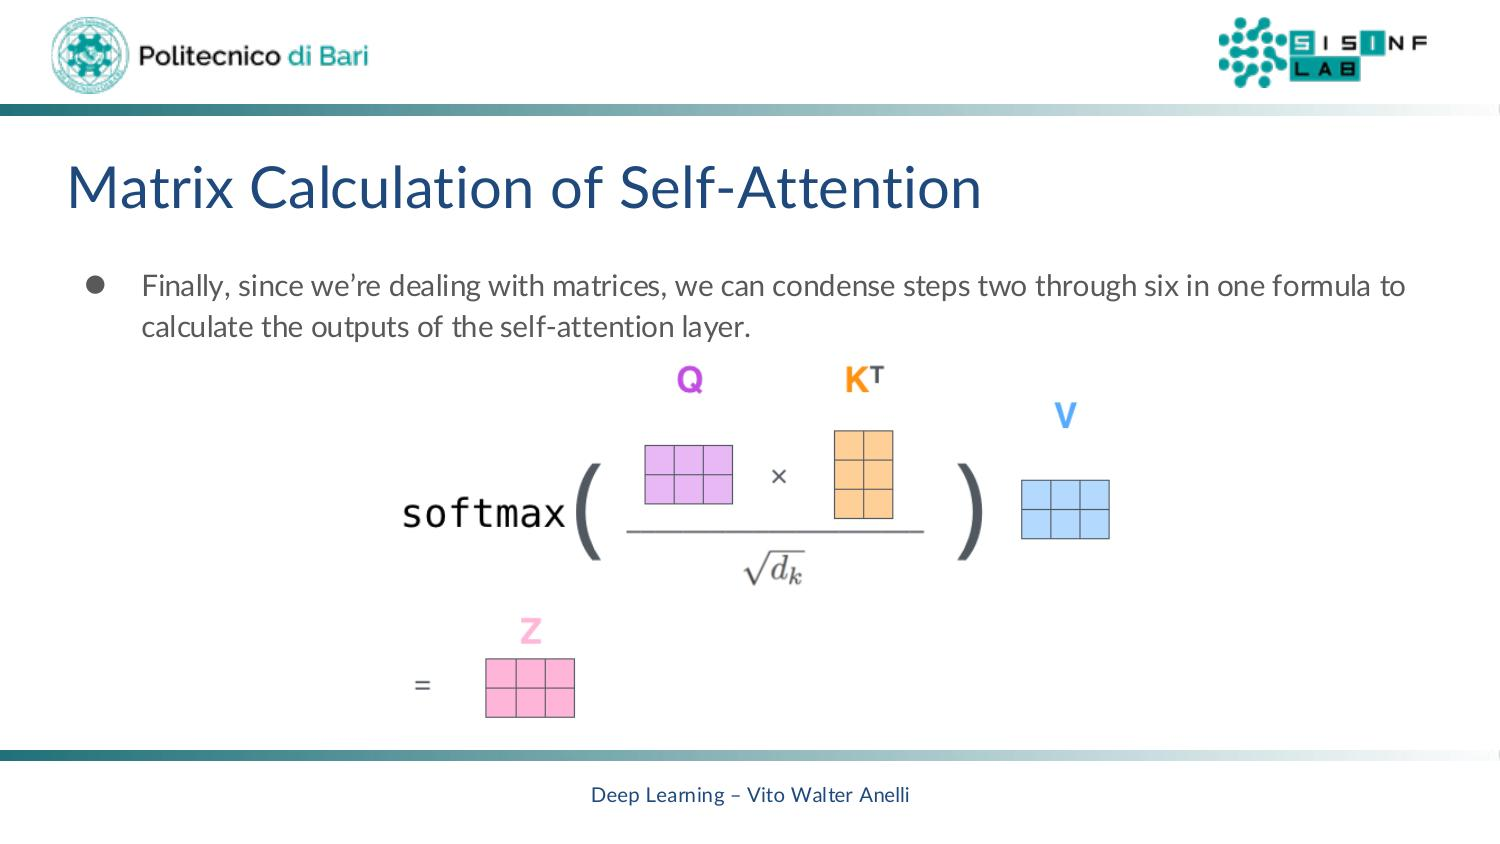
\includegraphics[width=0.62\linewidth]{figures/cf12_05_self_attn_formula.jpg}
  \caption{Formula matriciale della self-attention:
           $Z = \mathrm{softmax}(QK^\top/\sqrt{d_k})\,V$.
           $Q$ (viola) e $K^\top$ (arancione) sono $n \times 64$;
           $V$ (azzurro) e' $n \times 64$; $Z$ (rosa) e' $n \times 64$.}
  \label{fig:self_attn_formula}
\end{figure}

%------------------------------------------------------------
\section{Multi-Head Attention}
\label{sec:multihead}

L'attenzione \textbf{multi-head} (MHA) porta due vantaggi rispetto
alla singola testa:

\begin{enumerate}
  \item \textbf{Focus su posizioni diverse}: ogni testa si specializza
        su relazioni diverse (sintattiche, semantiche, posizionali).
  \item \textbf{Sottospazi multipli}: con $h$ teste si hanno $h$
        proiezioni indipendenti dello spazio semantico.
\end{enumerate}

Il paper originale usa $h = 8$ teste. Per ogni testa $i$ si
mantengono matrici separate $W_i^Q, W_i^K, W_i^V$ e si calcola
$Z_i$ con la formula~\eqref{eq:self-attn-matrix}. Poi:

\begin{equation}
  \mathrm{MHA}(Q,K,V) = \mathrm{Concat}(Z_0,\ldots,Z_7)\, W^O,
  \label{eq:mha}
\end{equation}

con $W^O \in \mathbb{R}^{h \cdot d_v \times d_{\text{model}}}$.

\begin{figure}[H]
  \centering
  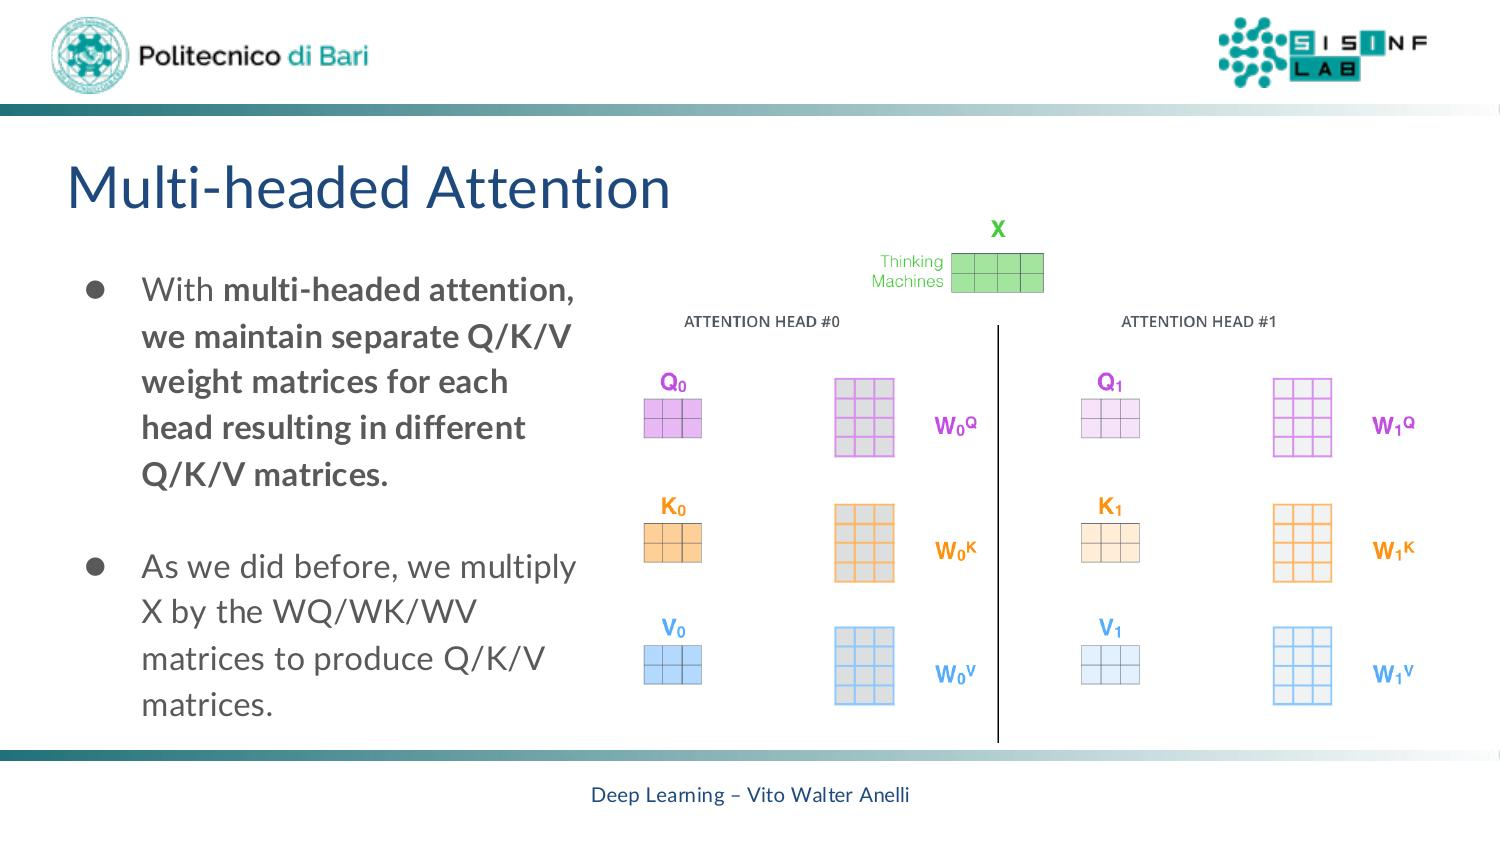
\includegraphics[width=0.82\linewidth]{figures/cf12_06_multihead_separate_qkv.jpg}
  \caption{Multi-head attention: set di pesi $W^Q$, $W^K$, $W^V$
           separati per ogni testa, producendo matrici Q, K, V
           distinte. Le due teste mostrate operano su diversi
           ``sottospazi di rappresentazione''.}
  \label{fig:multihead_qkv}
\end{figure}

\begin{figure}[H]
  \centering
  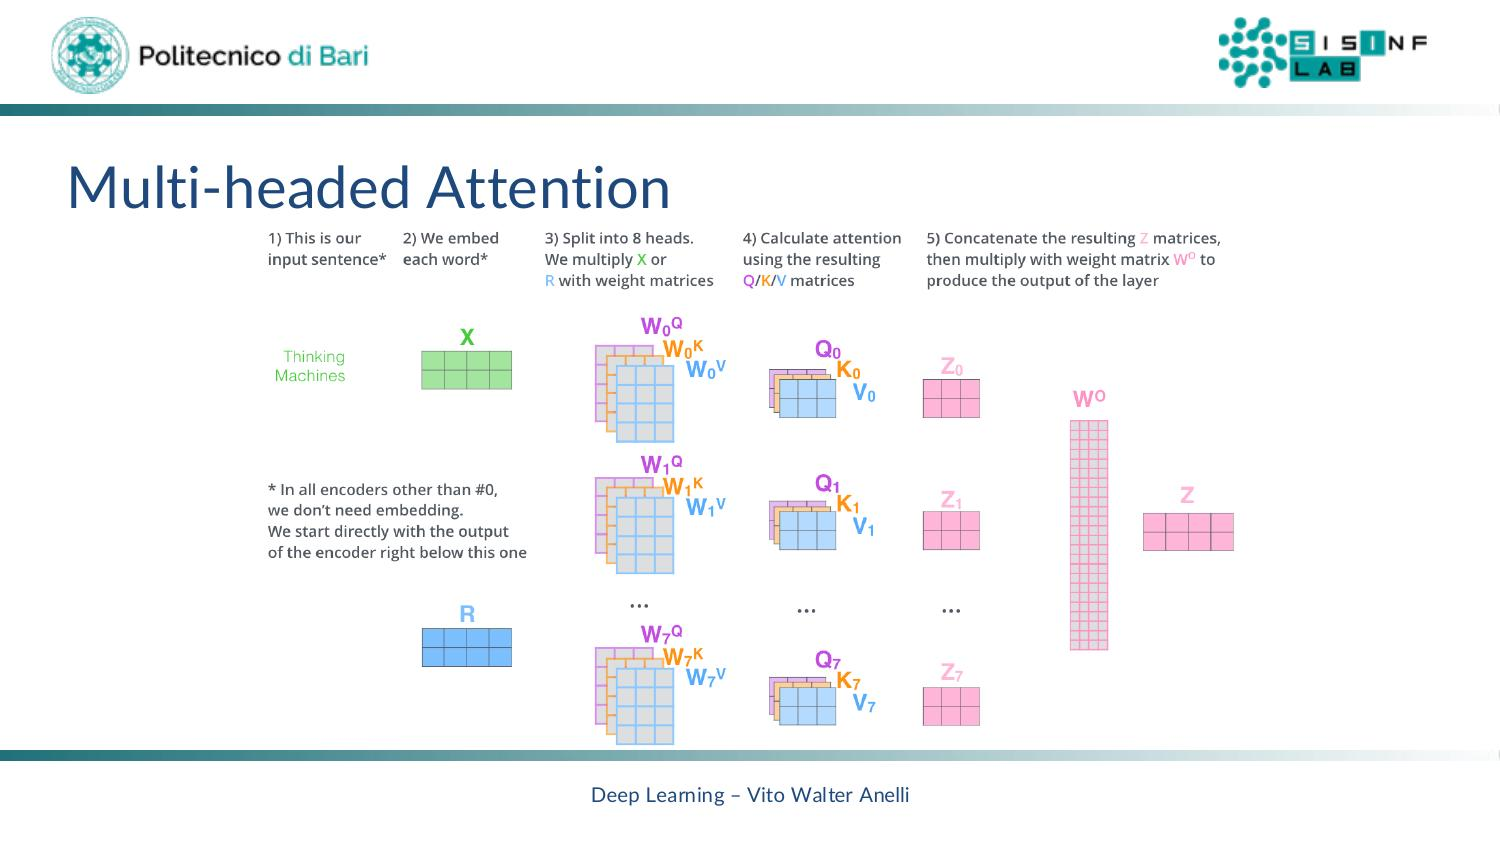
\includegraphics[width=0.95\linewidth]{figures/cf12_07_multihead_full_pipeline.jpg}
  \caption{Pipeline completa della Multi-Head Attention con $h=8$.
           (1) Frase di input. (2) Embedding. (3) Calcolo di
           $Q_i, K_i, V_i$ per ogni testa. (4) Calcolo di $Z_i$.
           (5) Concatenazione e proiezione con $W^O$.}
  \label{fig:multihead_pipeline}
\end{figure}

%------------------------------------------------------------
\section{Positional Encoding}
\label{sec:positional-encoding}

Il Transformer processa tutti i token in parallelo: senza segnale
di posizione, sarebbe invariante alla permutazione dei token.
Il \textbf{positional encoding} risolve il problema sommando un
vettore di posizione all'embedding:

\begin{figure}[H]
  \centering
  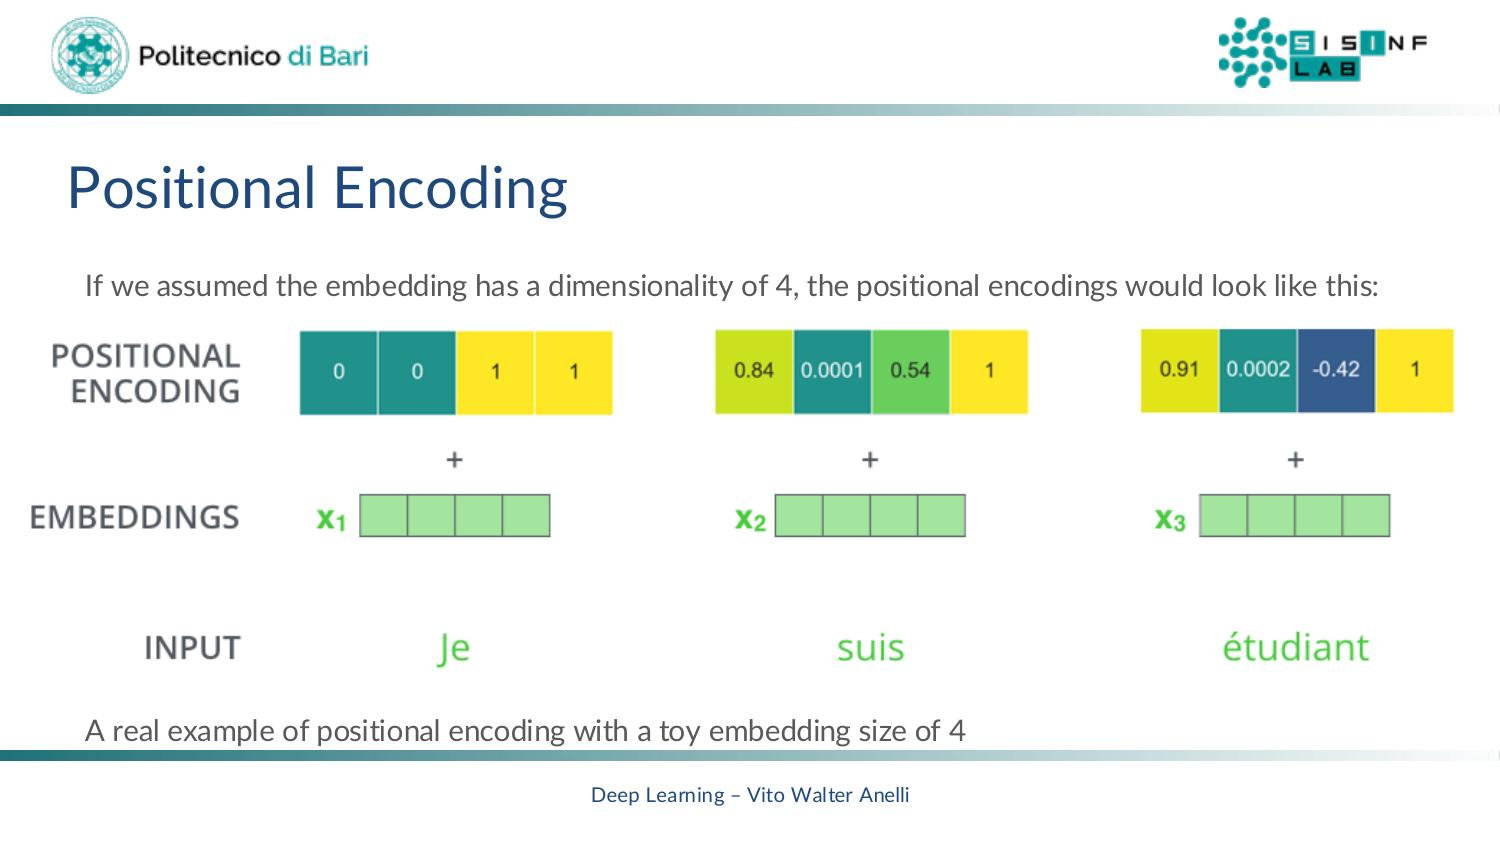
\includegraphics[width=0.88\linewidth]{figures/cf12_08_positional_encoding_example.jpg}
  \caption{Positional encoding con $d = 4$. Per ogni token si somma
           l'embedding $x_i$ al vettore PE corrispondente alla sua
           posizione. Posizioni diverse ricevono vettori diversi.}
  \label{fig:pe_example}
\end{figure}

La codifica sinusoidale deterministica del paper e':

\begin{align}
  \mathrm{PE}(pos,\, 2i)   &= \sin\!\left(\tfrac{pos}{10000^{2i/d_{\text{model}}}}\right),
  \label{eq:pe-sin}\\[4pt]
  \mathrm{PE}(pos,\, 2i+1) &= \cos\!\left(\tfrac{pos}{10000^{2i/d_{\text{model}}}}\right),
  \label{eq:pe-cos}
\end{align}

dove $pos$ e' la posizione e $i$ indicizza la dimensione. Le frequenze
variano geometricamente, permettendo di apprendere relazioni posizionali
relative a qualsiasi distanza. Non introduce parametri aggiuntivi e
generalizza a sequenze piu' lunghe di quelle di training.

\begin{figure}[H]
  \centering
  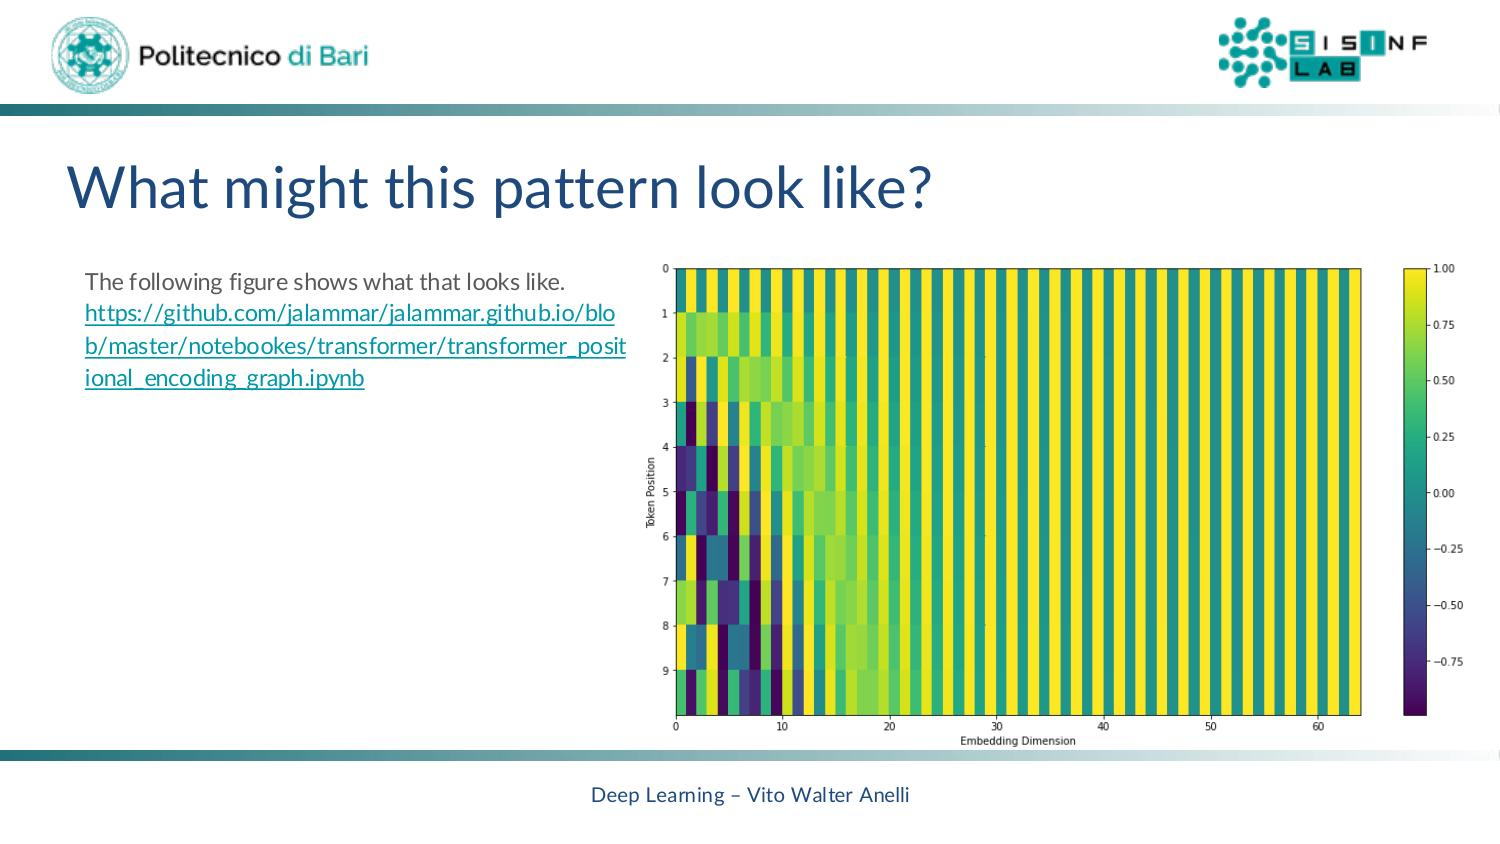
\includegraphics[width=0.72\linewidth]{figures/cf12_09_pe_heatmap.jpg}
  \caption{Heatmap dei vettori di PE ($y$: posizione del token,
           $x$: dimensione dell'embedding). Le prime dimensioni hanno
           alta frequenza (pattern fitto), le ultime bassa frequenza
           (pattern lento). Ogni riga e' il vettore PE per quella
           posizione.}
  \label{fig:pe_heatmap}
\end{figure}

%------------------------------------------------------------
\section{Residual Connections e Layer Normalization}
\label{sec:residuals}

Ogni sotto-livello e' avvolto da una \textbf{connessione residuale}
seguita da \textbf{layer normalization}:

\begin{equation}
  \mathbf{y} = \mathrm{LayerNorm}\!\left(\mathbf{x}
               + \mathrm{Sublayer}(\mathbf{x})\right).
  \label{eq:residual}
\end{equation}

Le connessioni residuali mitigano il vanishing gradient nelle reti
profonde. La layer normalization normalizza su ciascun esempio
(non sul batch), risultando piu' adatta alle sequenze di lunghezza
variabile rispetto alla batch normalization.

\begin{figure}[H]
  \centering
  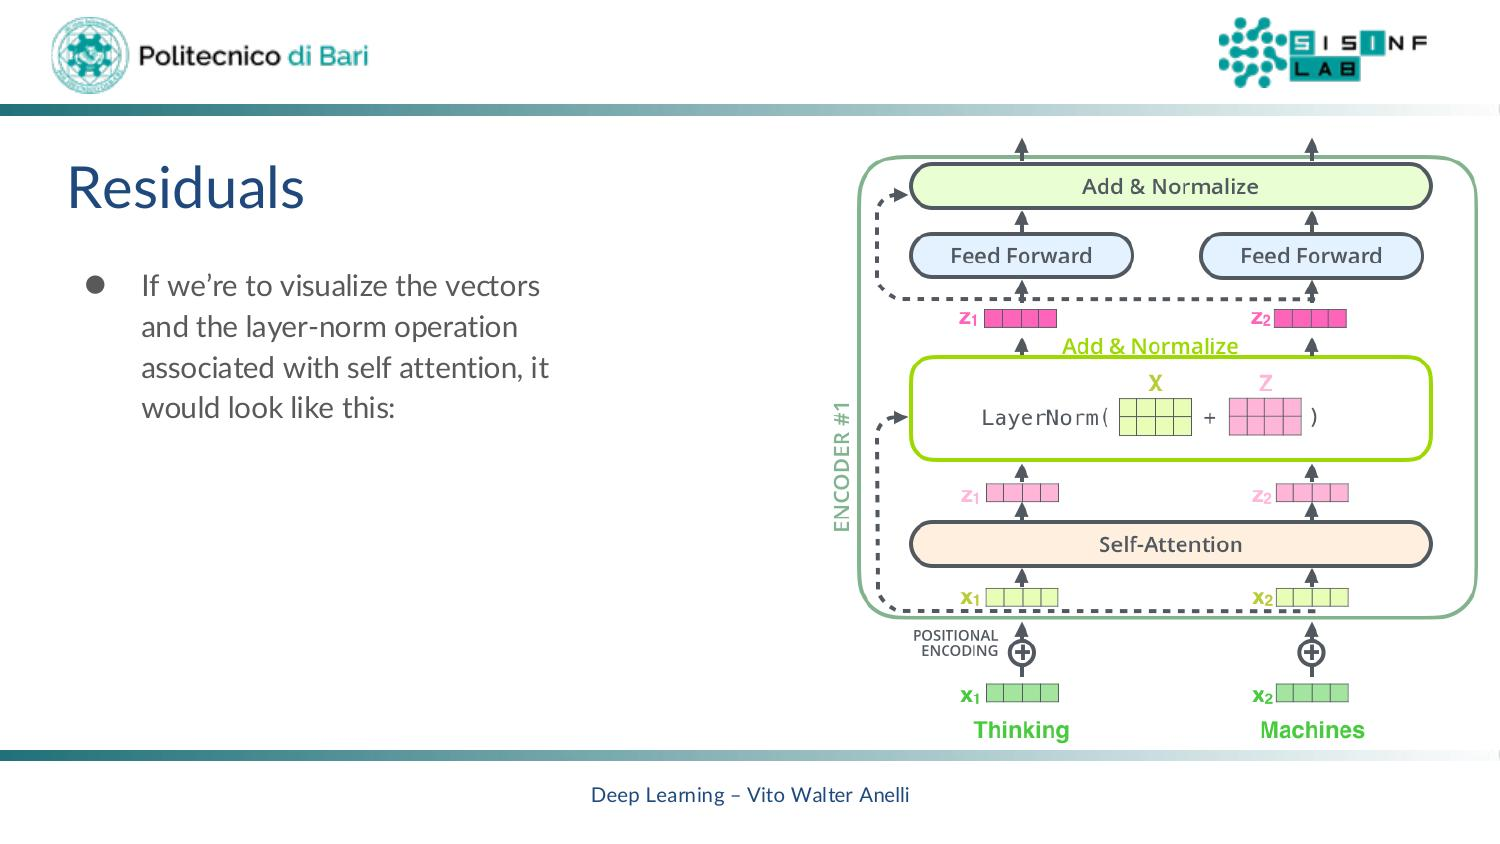
\includegraphics[width=0.62\linewidth]{figures/cf12_10_residuals_layernorm.jpg}
  \caption{Encoder con residual connections e layer normalization.
           I vettori $x_1, x_2$ (con PE sommato) attraversano
           Self-Attention producendo $z_1, z_2$; si applica
           $\mathrm{LayerNorm}(x + z)$; poi FFN con un secondo
           Add \& Normalize.}
  \label{fig:residuals_layernorm}
\end{figure}

%------------------------------------------------------------
\section{Lato Decoder}
\label{sec:decoder}

\subsection{Encoder-Decoder Attention e Generazione}
\label{subsec:dec-operation}

Il top encoder produce K e V che alimentano l'Encoder-Decoder
Attention di ogni decoder block; le Q provengono dal decoder stesso.
La generazione e' autoregressiva: al passo $t$ il decoder riceve
la sequenza generata fino a $t-1$ e produce la distribuzione su $w_t$.

\begin{figure}[H]
  \centering
  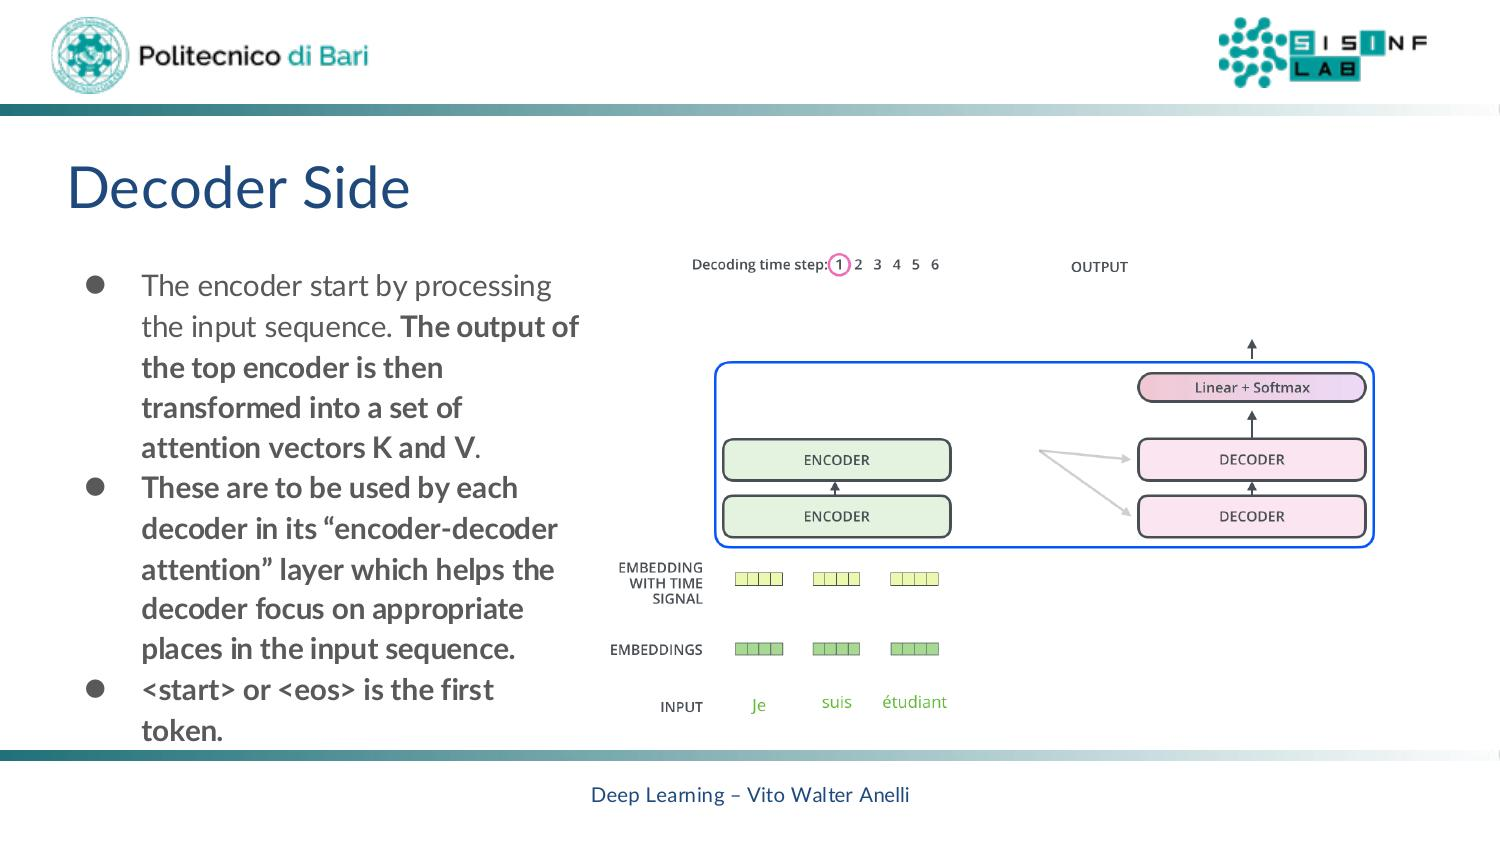
\includegraphics[width=0.82\linewidth]{figures/cf12_11_decoder_side.jpg}
  \caption{Lato decoder: K e V dell'encoder alimentano ogni decoder
           block. La generazione avviene passo per passo (time step
           1, 2, \ldots); ogni token prodotto viene rialimentato
           come input del passo successivo.}
  \label{fig:decoder_side}
\end{figure}

La masked self-attention garantisce la causalita' imponendo:

\begin{equation}
  \tilde{S}_{ij} = \begin{cases}
    S_{ij}  & j \le i,\\
    -\infty & j > i.
  \end{cases}
  \label{eq:attn-mask}
\end{equation}

\subsection{Strato Lineare e Softmax Finale}
\label{subsec:linear-softmax}

Il vettore di output del decoder ($d_{\text{model}}$ dim) viene
proiettato su $|\mathcal{V}|$ logit da uno strato lineare, poi
una softmax produce la distribuzione:

\begin{equation}
  P(w) = \frac{e^{\ell_w}}{\sum_{w'} e^{\ell_{w'}}}.
  \label{eq:output-softmax}
\end{equation}

\begin{figure}[H]
  \centering
  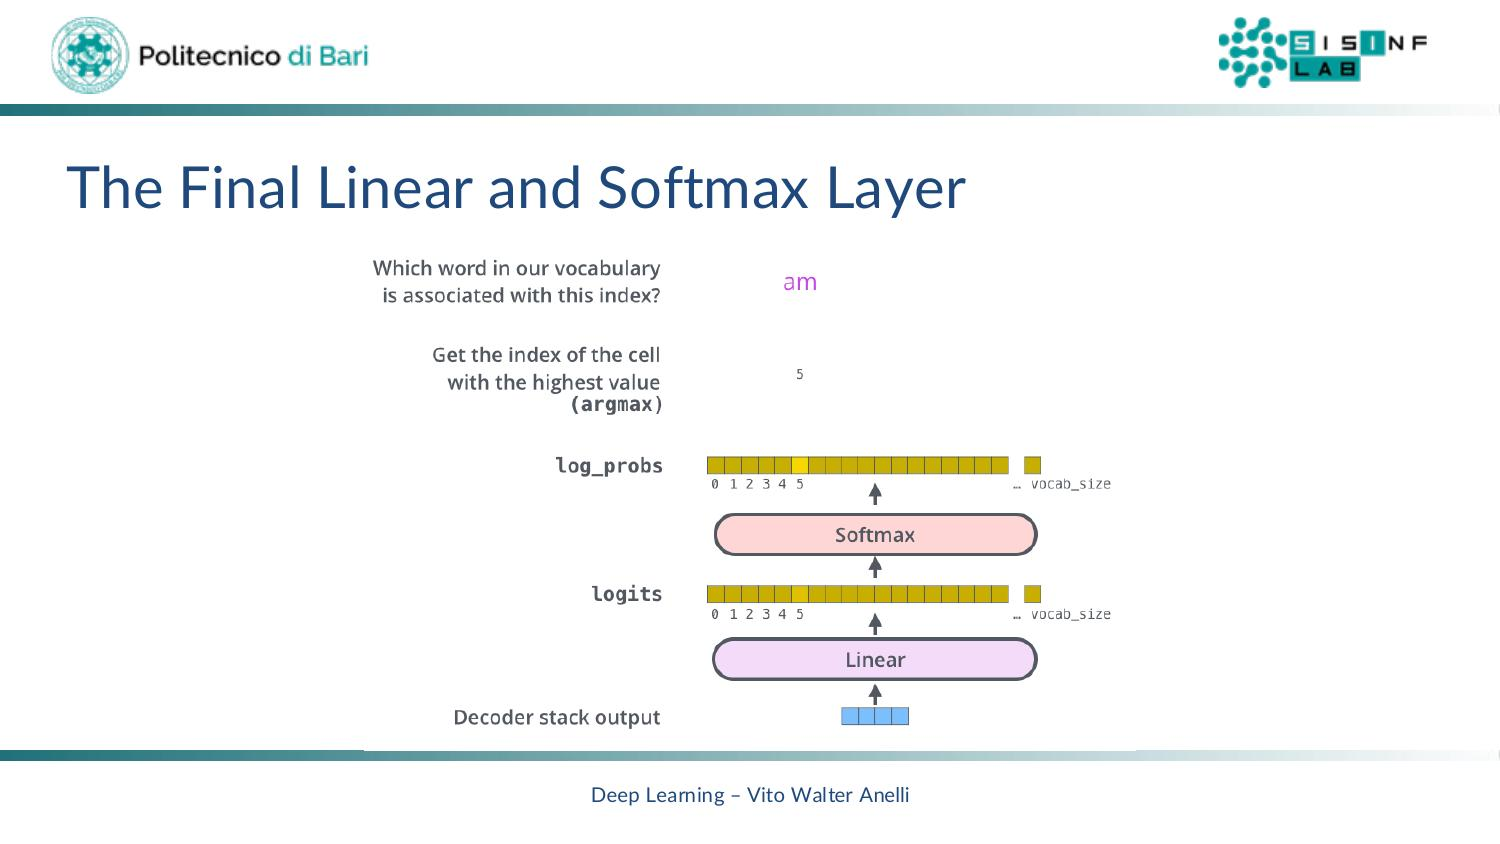
\includegraphics[width=0.56\linewidth]{figures/cf12_12_linear_softmax.jpg}
  \caption{Pipeline di output: il decoder stack output passa attraverso
           lo strato lineare (logits, dim $= |\mathcal{V}|$), poi la
           softmax produce le log-probabilita'. L'argmax sull'indice
           restituisce il token predetto (es.\ ``am'' all'indice 5).}
  \label{fig:linear_softmax}
\end{figure}

%------------------------------------------------------------
\section{Addestramento del Transformer}
\label{sec:training}

Durante il training si usa il \emph{teacher forcing}: il decoder
riceve l'intera sequenza target shiftata di una posizione a destra
(\texttt{<start>}, $w_1^*, w_2^*, \ldots$). La masked self-attention
garantisce che la posizione $t$ non veda i token successivi.

La loss e' la cross-entropy media su tutte le posizioni:

\begin{equation}
  \mathcal{L} = -\frac{1}{T}\sum_{t=1}^{T}
                \log P\!\left(w_t^* \mid w_1^*, \ldots, w_{t-1}^*\right).
  \label{eq:loss}
\end{equation}

%------------------------------------------------------------
\section{BERT}
\label{sec:bert}

\subsection{Architettura}
\label{subsec:bert-arch}

BERT (\emph{Bidirectional Encoder Representations from Transformers})
usa solo lo stack di encoder senza decoder. Essendo non causale,
ogni token puo' attendere a tutti gli altri in entrambe le direzioni
(\emph{bidirezionale}). Le due varianti principali sono:

\begin{itemize}
  \item \textbf{BERT Base}: 12 layer, $d_{\text{model}} = 768$,
        12 teste, 110M parametri.
  \item \textbf{BERT Large}: 24 layer, $d_{\text{model}} = 1024$,
        16 teste, 340M parametri.
\end{itemize}

Il primo token e' sempre \texttt{[CLS]} (\emph{classification}): il
suo vettore di output aggrega informazione globale sulla sequenza ed
e' usato per i task di classificazione.

\begin{figure}[H]
  \centering
  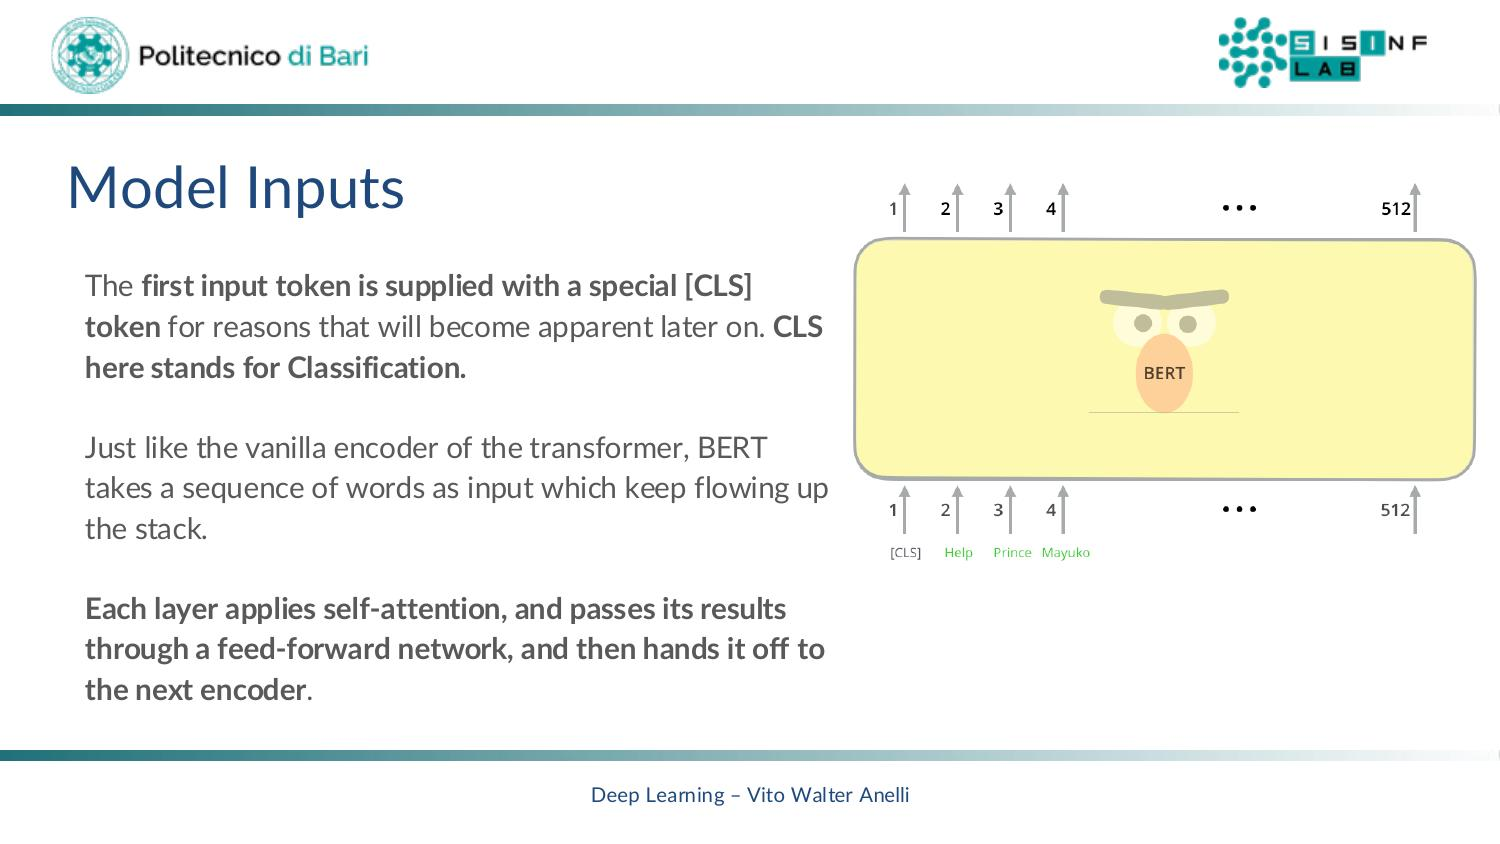
\includegraphics[width=0.70\linewidth]{figures/cf12_13_bert_inputs.jpg}
  \caption{Input di BERT: la sequenza inizia con \texttt{[CLS]},
           seguita dai token della frase. I 12 encoder layer
           producono un vettore di output per ogni posizione.}
  \label{fig:bert_inputs}
\end{figure}

\begin{figure}[H]
  \centering
  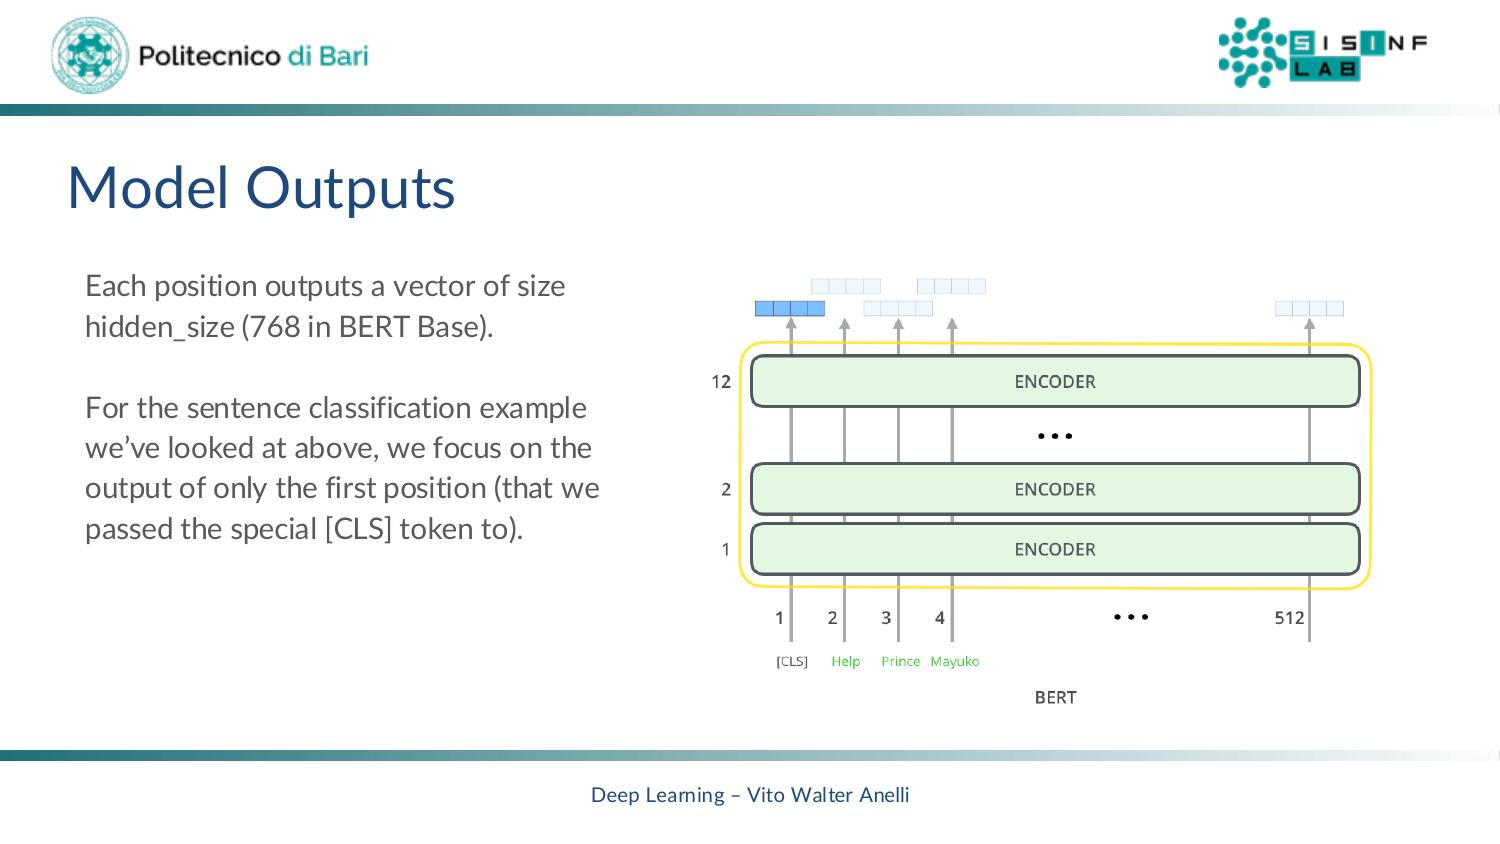
\includegraphics[width=0.70\linewidth]{figures/cf12_14_bert_outputs.jpg}
  \caption{Output di BERT per la classificazione. Ogni posizione
           produce un vettore di 768 dim. Per task a livello di frase
           si usa solo il vettore \texttt{[CLS]} (posizione 1),
           passato a un classificatore lineare + softmax.}
  \label{fig:bert_outputs}
\end{figure}

\subsection{Pre-training}
\label{subsec:bert-pretrain}

\begin{description}
  \item[Masked Language Model (MLM)] Il 15\% dei token viene
        selezionato: l'80\% sostituito con \texttt{[MASK]}, il 10\%
        con token casuale, il 10\% lasciato invariato. Il modello
        deve predire il token originale.
  \item[Next Sentence Prediction (NSP)] Il modello decide se la
        frase B segue naturalmente la frase A nel testo originale.
\end{description}

\subsection{Utilizzo}
\label{subsec:bert-use}

\begin{description}
  \item[Fine-tuning] Si aggiunge un classificatore sul vettore
        \texttt{[CLS]} e si ri-addestra l'intero modello con
        learning rate ridotto.
  \item[Feature extraction] BERT e' congelato; i vettori contestuali
        sono usati come features per un modello esterno. La
        combinazione degli ultimi 4 layer raggiunge risultati
        vicini al fine-tuning su task come NER.
\end{description}

%------------------------------------------------------------
\section{GPT}
\label{sec:gpt}

\subsection{Architettura Decoder-Only}
\label{subsec:gpt-arch}

GPT (\emph{Generative Pretrained Transformer}) usa solo lo stack di
decoder (\emph{decoder-only}): l'Encoder-Decoder Attention viene
rimosso; ogni blocco ha solo Masked Self-Attention + FFN. Il modello
e' autoregressivo: genera un token alla volta condizionandosi su
tutti quelli precedenti.

\subsection{Masked Self-Attention: Dettaglio Numerico}
\label{subsec:masked-sa}

\begin{figure}[H]
  \centering
  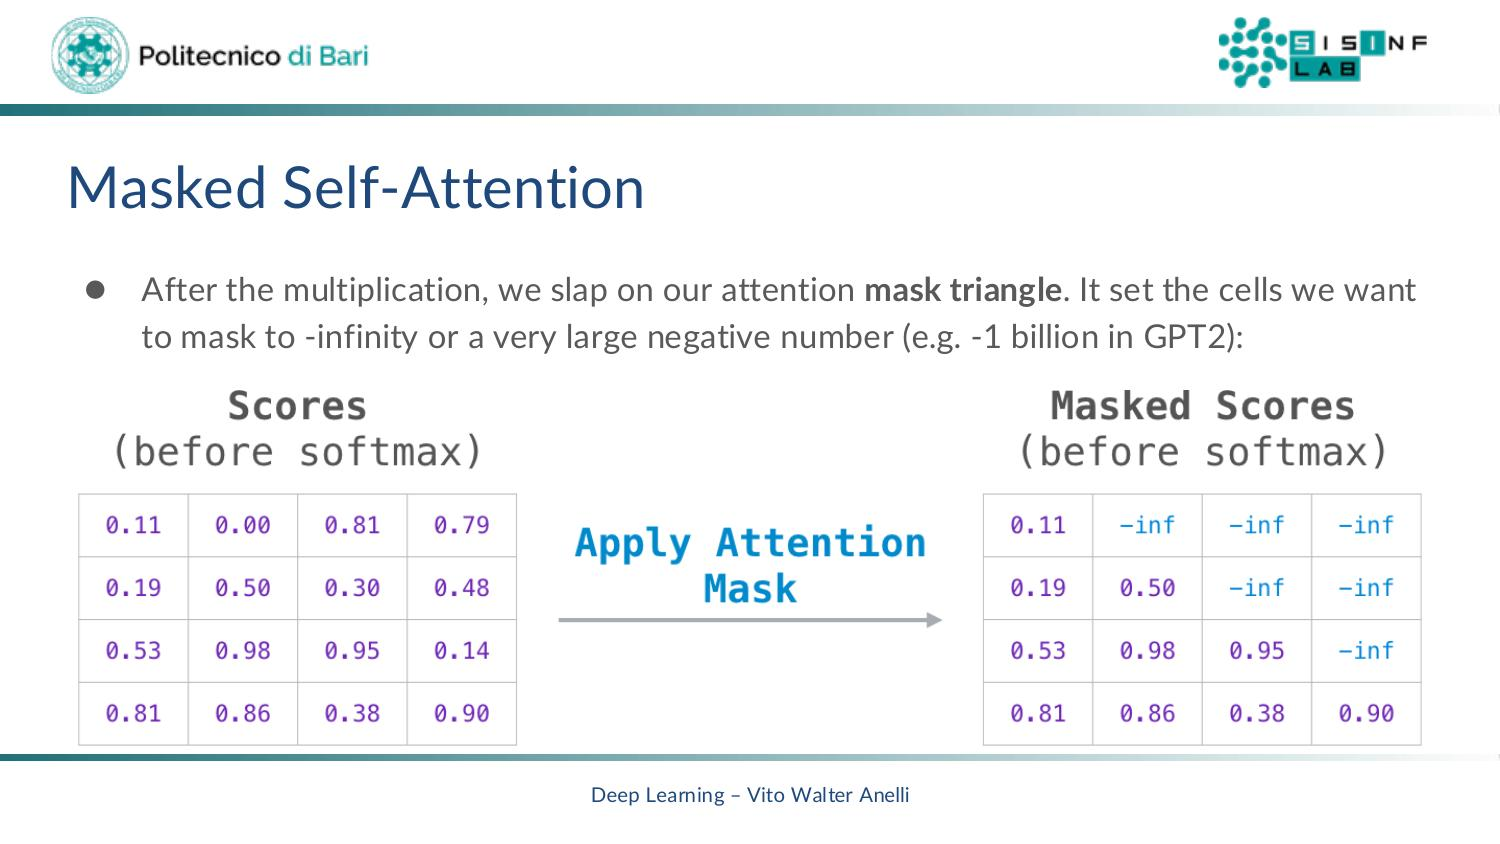
\includegraphics[width=0.88\linewidth]{figures/cf12_16_masked_attn_triangle.jpg}
  \caption{Applicazione della maschera triangolare. Sinistra: score
           originali. Destra: score mascherati con $-\infty$ nelle
           posizioni future (triangolo superiore). La riga $i$ puo'
           attendere solo alle colonne $j \le i$.}
  \label{fig:masked_triangle}
\end{figure}

\begin{figure}[H]
  \centering
  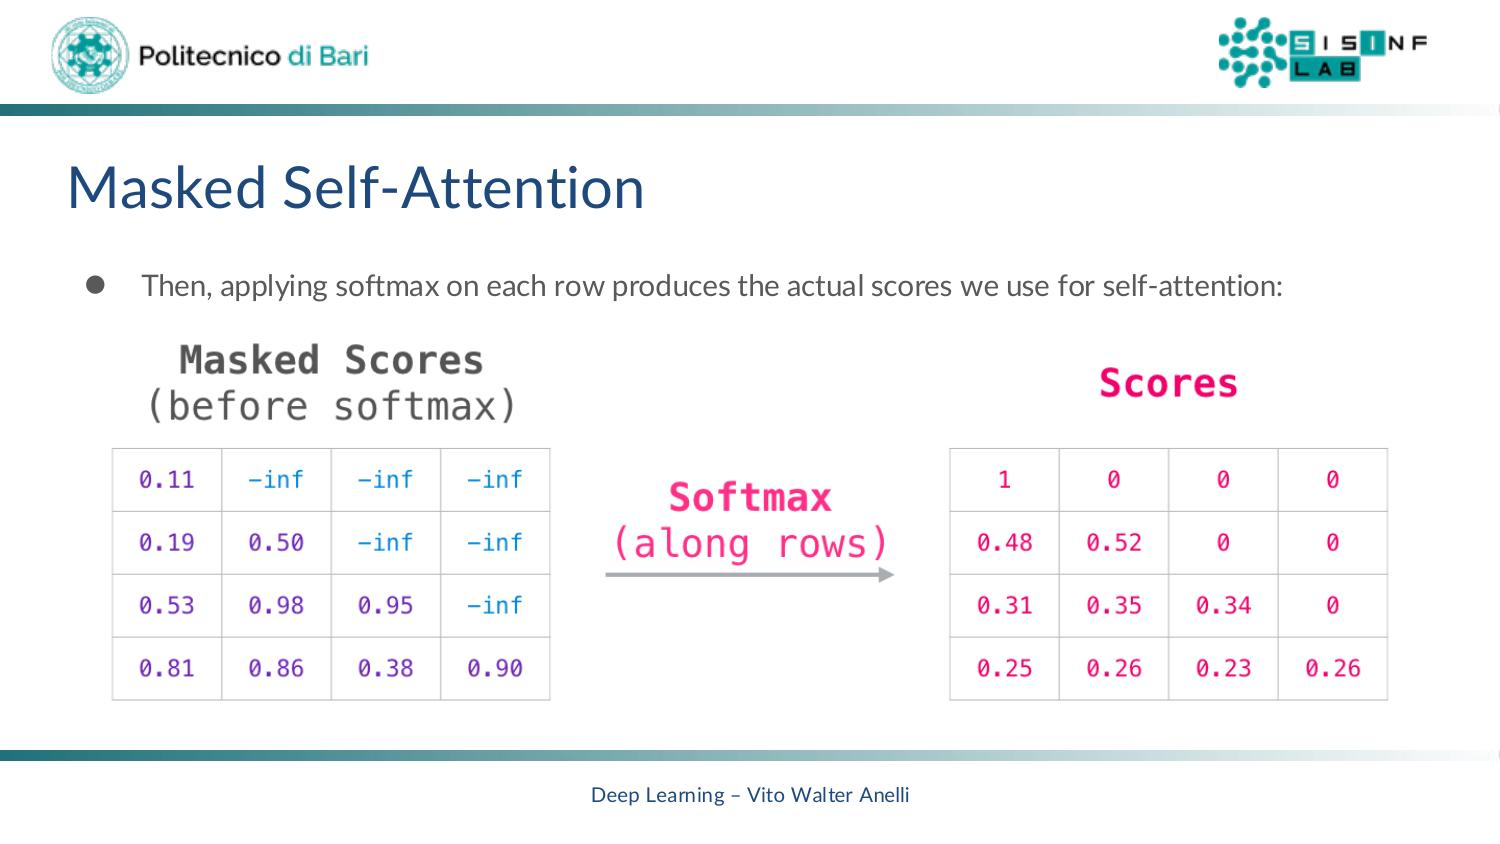
\includegraphics[width=0.88\linewidth]{figures/cf12_17_masked_attn_softmax.jpg}
  \caption{Dopo la softmax per righe, i valori $-\infty$ diventano 0.
           La prima riga attende solo se stessa $(1, 0, 0, 0)$;
           la quarta puo' attendere a tutti e 4 i token.}
  \label{fig:masked_softmax}
\end{figure}

\subsection{Decoder Block e Generazione}
\label{subsec:gpt-gen}

\begin{figure}[H]
  \centering
  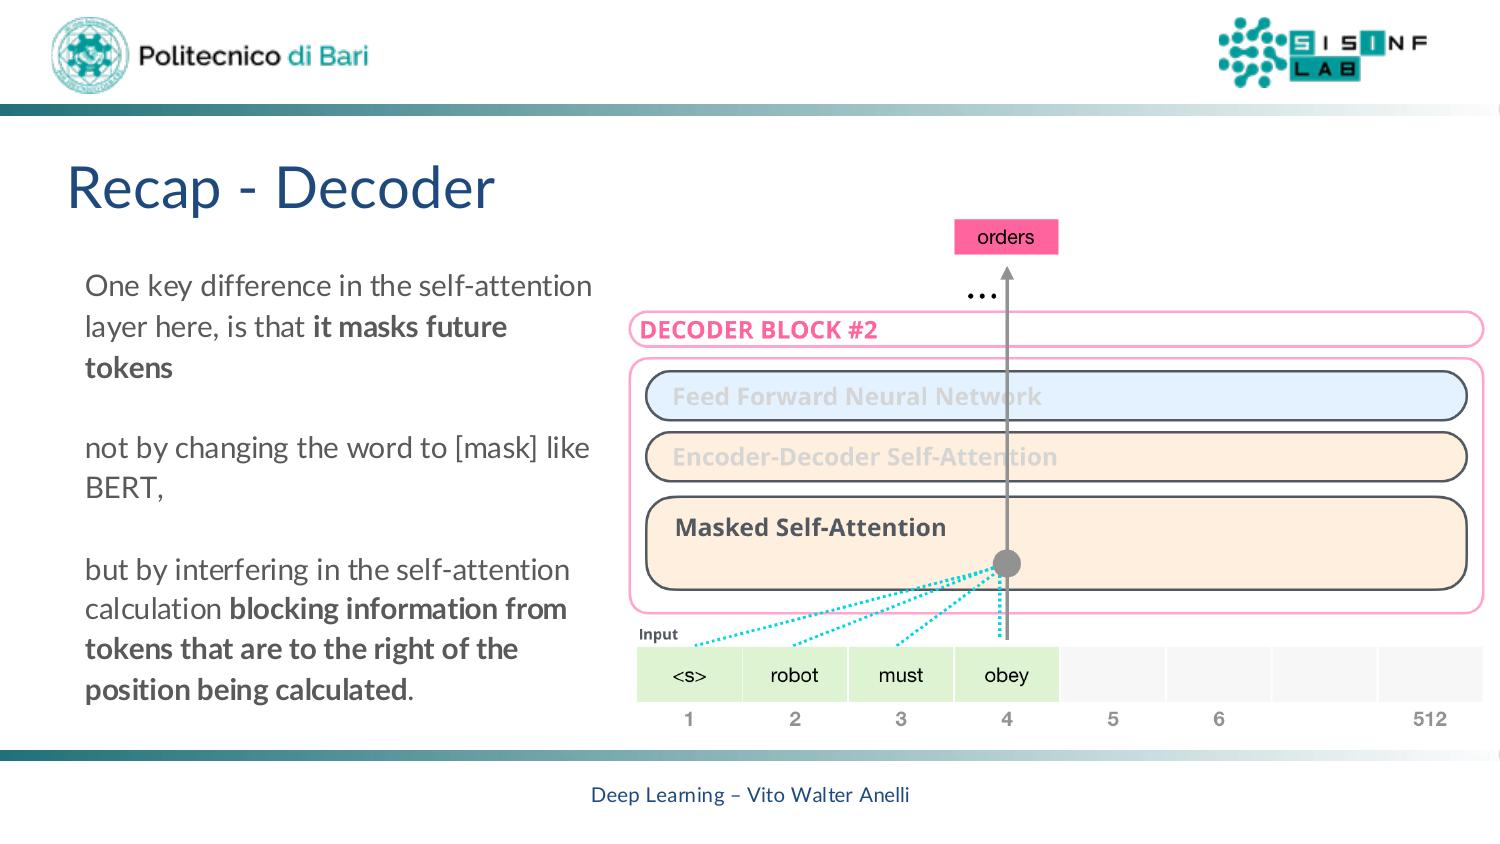
\includegraphics[width=0.82\linewidth]{figures/cf12_15_decoder_masked_recap.jpg}
  \caption{Decoder block di GPT: il Masked Self-Attention blocca le
           informazioni dai token alla destra della posizione corrente
           interferendo nel calcolo degli score, non sostituendo i
           token con \texttt{[MASK]} come BERT.}
  \label{fig:decoder_masked}
\end{figure}

Durante l'inferenza GPT genera un token alla volta (\emph{auto-regressione}).
La \textbf{KV cache} conserva le chiavi e i valori dei token gia'
elaborati, evitando il ricalcolo completo ad ogni passo.
Il parametro \textbf{top-k} controlla la varieta': con $k=1$ si usa
il token piu' probabile (greedy); con $k > 1$ si campiona tra i $k$
piu' probabili.

\subsection{Pipeline Self-Attention in GPT-2 Small}
\label{subsec:gpt2-pipeline}

GPT-2 Small: $h = 12$ teste, $d_{\text{model}} = 768$, $d_k = 64$.

\begin{description}
  \item[Fase 1 -- q, k, v] Il vettore di input (768) e' moltiplicato
        per una matrice $768 \times 2304$, ottenendo per
        concatenazione i vettori q, k, v (768 dim ciascuno).
  \item[Fase 1.5 -- Split] q (e analogamente k, v) viene rimodellato
        in $12 \times 64$: una riga per testa.
\end{description}

\begin{figure}[H]
  \centering
  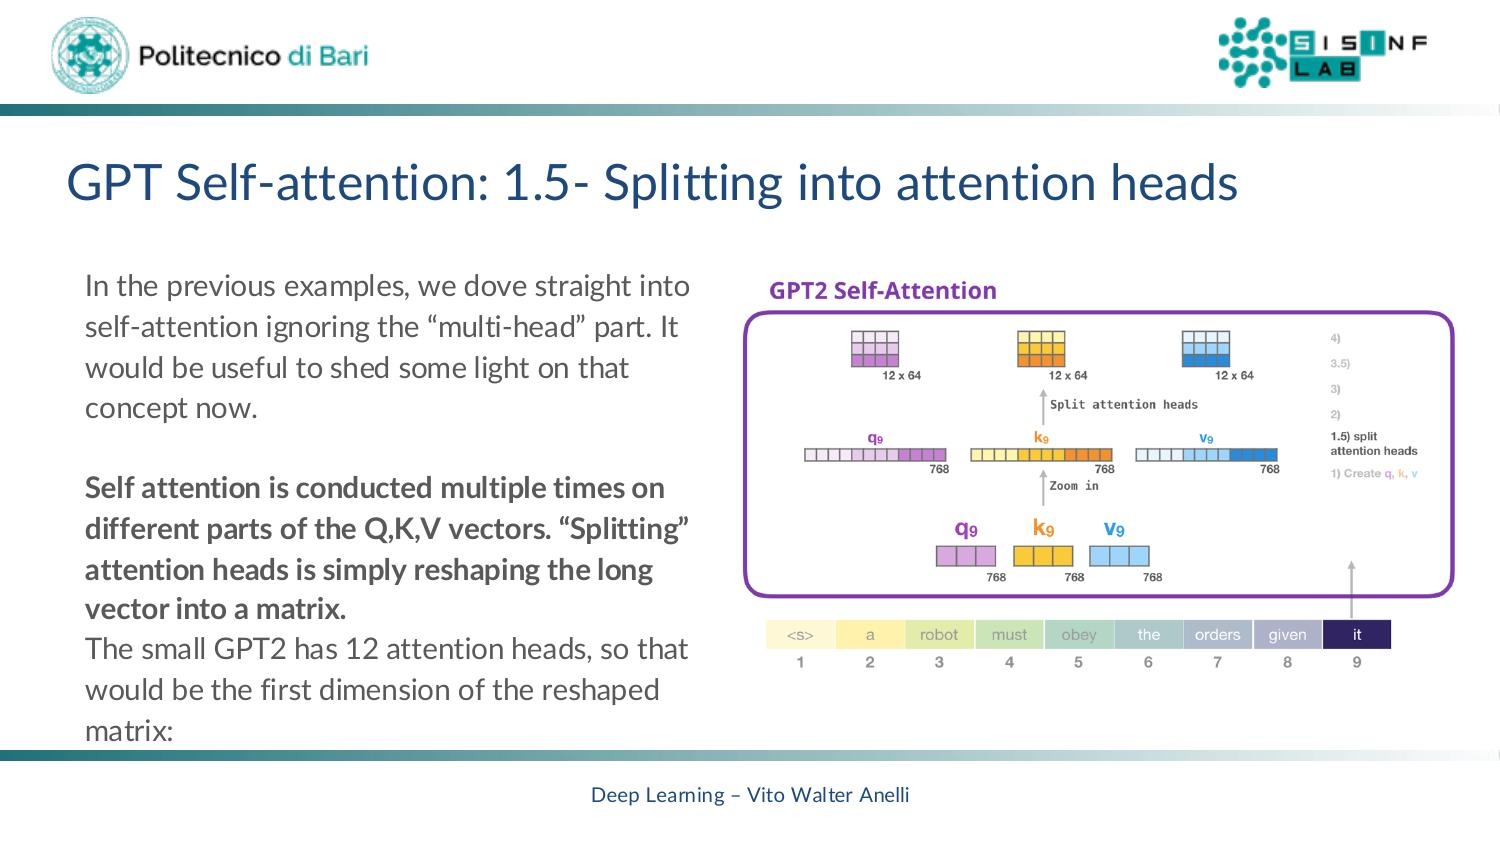
\includegraphics[width=0.85\linewidth]{figures/cf12_18_gpt_head_split.jpg}
  \caption{Split delle teste in GPT-2. I vettori q, k, v di 768 dim
           sono rimodellati in matrici $12 \times 64$. Ogni testa opera
           su 64 dimensioni della rappresentazione originale.}
  \label{fig:head_split}
\end{figure}

\begin{description}
  \item[Fase 2 -- Scoring] Ogni testa calcola il prodotto scalare
        tra la propria query e le chiavi di tutti i token precedenti
        (KV cache), scalato per $\sqrt{64}$.
  \item[Fase 3 -- Somma] I value sono pesati dagli score softmaxati
        e sommati.
  \item[Fase 3.5 -- Merge] I 12 vettori di output sono concatenati
        (768 dim totali).
  \item[Fase 4 -- Proiezione] Il vettore concatenato e' proiettato
        da $W^O \in \mathbb{R}^{768 \times 768}$ per produrre
        l'output della self-attention.
\end{description}

\begin{figure}[H]
  \centering
  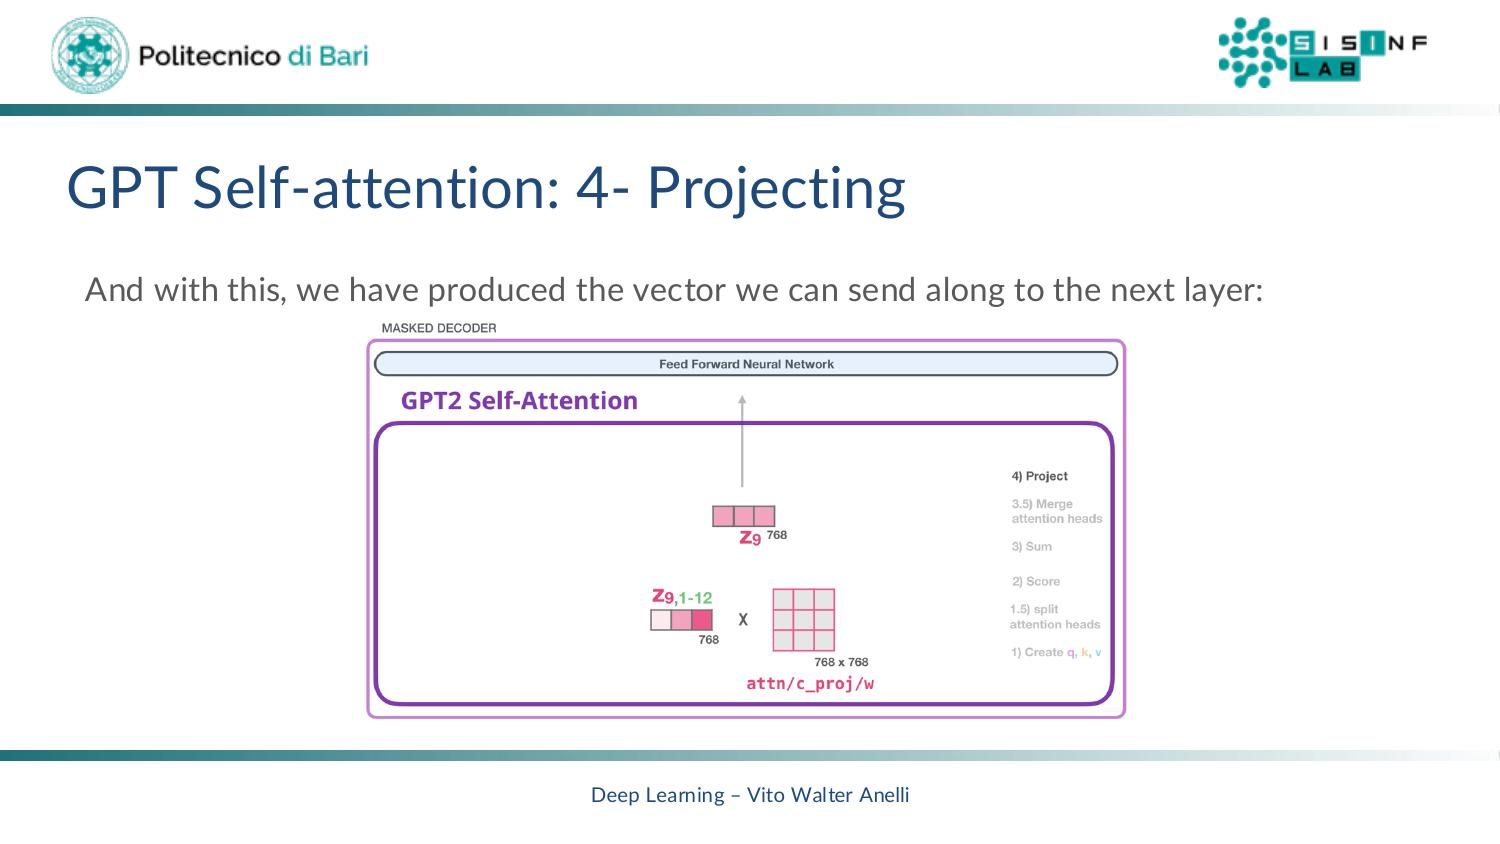
\includegraphics[width=0.70\linewidth]{figures/cf12_19_gpt_projection.jpg}
  \caption{Fase 4: il vettore $Z_{9,1\text{-}12}$ (768 dim,
           concatenazione delle 12 teste) e' proiettato da
           $W^O$ ($768 \times 768$) producendo $Z_9$ (768 dim),
           che passa al FFN del blocco.}
  \label{fig:gpt_proj}
\end{figure}

\subsection{Matrici di Peso in GPT-2 Small}
\label{subsec:gpt2-weights}

\begin{figure}[H]
  \centering
  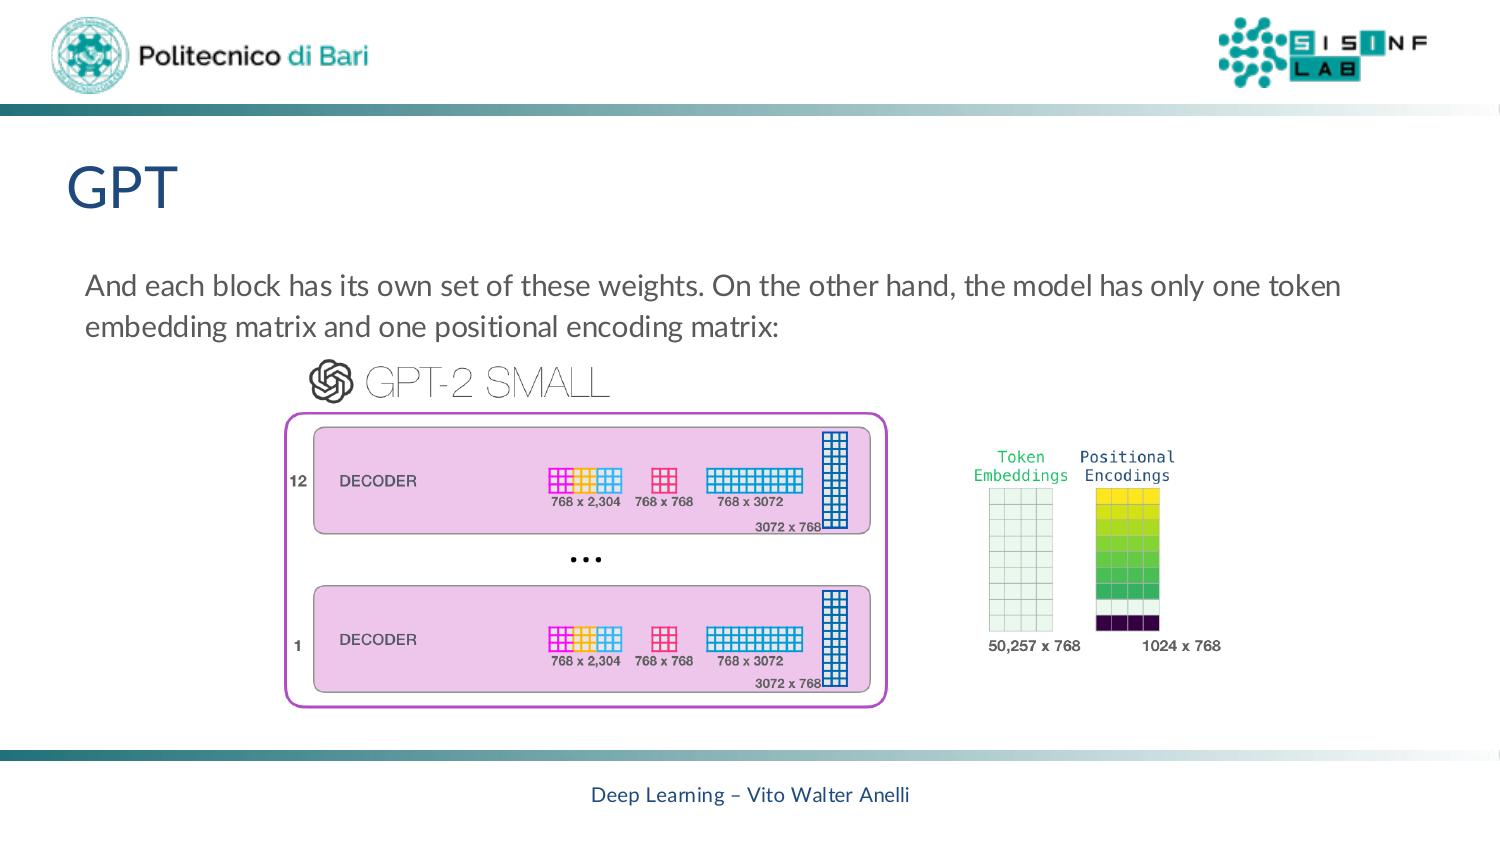
\includegraphics[width=0.88\linewidth]{figures/cf12_20_gpt2_weight_matrices.jpg}
  \caption{Matrici di peso di GPT-2 Small. Ogni decoder block ha:
           $768 \times 2304$ (Q/K/V), $768 \times 768$ (proiezione
           attenzione), $768 \times 3072$ e $3072 \times 768$ (FFN).
           Il modello condivide una sola matrice di token embedding
           ($50257 \times 768$) e una di positional encoding
           ($1024 \times 768$).}
  \label{fig:gpt2_weights}
\end{figure}

Il FFN interno a ogni blocco applica:

\begin{equation}
  \mathrm{FFN}(\mathbf{x})
    = \mathrm{GELU}(\mathbf{x}\,W_1 + b_1)\,W_2 + b_2,
  \label{eq:ffn}
\end{equation}

con $W_1 \in \mathbb{R}^{768 \times 3072}$ e
$W_2 \in \mathbb{R}^{3072 \times 768}$
(dimensione interna $= 4 \times d_{\text{model}}$).

%------------------------------------------------------------
\section{BERT vs.\ GPT: Confronto}
\label{sec:bert-gpt}

\begin{table}[H]
  \centering
  \caption{Confronto tra BERT e GPT.}
  \label{tab:bert-gpt}
  \small
  \begin{tabular}{lll}
    \toprule
    \textbf{Caratteristica} & \textbf{BERT} & \textbf{GPT} \\
    \midrule
    Blocchi usati         & Solo encoder            & Solo decoder \\
    Direzione attenzione  & Bidirezionale           & Causale (sx) \\
    Paradigma             & Fill-in-the-blank (MLM) & Autoregressivo \\
    Pre-training          & MLM + NSP               & Language modeling \\
    Uso principale        & Comprensione (NLU)      & Generazione (NLG) \\
    Autoregressivo        & No                      & Si \\
    \bottomrule
  \end{tabular}
\end{table}

BERT eccelle nei task di comprensione in cui il contesto bilaterale
e' disponibile. GPT e' naturale per la generazione. Architetture
ibride come T5 e BART combinano entrambi gli stack.

%------------------------------------------------------------
\section{Riepilogo delle Componenti}
\label{sec:summary}

\begin{table}[H]
  \centering
  \caption{Componenti principali del Transformer.}
  \label{tab:components}
  \small
  \begin{tabular}{p{4.2cm}p{9cm}}
    \toprule
    \textbf{Componente} & \textbf{Funzione} \\
    \midrule
    Token Embedding
      & Mappa ogni token in $\mathbb{R}^{d_{\text{model}}}$. \\[2pt]
    Positional Encoding
      & Sinusoidi a frequenze diverse; nessun parametro extra. \\[2pt]
    Self-Attention (scalata)
      & $\mathrm{softmax}(QK^\top/\sqrt{d_k})\,V$. \\[2pt]
    Multi-Head Attention
      & $h$ teste in parallelo, concat + proiezione $W^O$. \\[2pt]
    Masked Self-Attention
      & Come SA ma con maschera causale ($-\infty$ per $j > i$). \\[2pt]
    Encoder-Decoder Attention
      & Q dal decoder, K e V dall'encoder. \\[2pt]
    Feed-Forward Network
      & Due layer lineari con GELU, per-posizione. \\[2pt]
    Residual + LayerNorm
      & $\mathrm{LayerNorm}(x + \mathrm{Sublayer}(x))$. \\[2pt]
    Linear + Softmax output
      & Proiezione sul vocabolario e distribuzione di probabilita'. \\
    \bottomrule
  \end{tabular}
\end{table}
